% Research draft; measured evidence is pinned in data/refresh20260927.
\documentclass[10pt,twocolumn,letterpaper]{article}
\usepackage[review]{cvpr}
\usepackage{amsmath,amssymb,graphicx,microtype,booktabs}
% Standard figure* floats; the legacy cuted teaser preamble is not needed.
\definecolor{cvprblue}{rgb}{0.21,0.49,0.74}
\usepackage[pagebackref,breaklinks,colorlinks,allcolors=cvprblue]{hyperref}
\hypersetup{pdftitle={RegLIC: Region-Adaptive Learned Image Compression},pdfauthor={Anonymous research draft},pdfsubject={DCVC-UF intra spatial early exit}}
\def\paperID{DRAFT}
\def\confName{CVPR}
\def\confYear{2027}
% Generated by scripts/paper_refresh_data.py; do not edit.
\newcommand{\TightOracleSaving}{20.90}
\newcommand{\TightRouterSaving}{17.15}
\newcommand{\TightDitherSaving}{14.90}
\newcommand{\TightUniformSaving}{10.48}
\newcommand{\TightPremium}{2.26}
\newcommand{\TightPremiumLow}{1.55}
\newcommand{\TightPremiumHigh}{2.99}
\newcommand{\TightN}{204}
\newcommand{\MainOracleSaving}{29.52}
\newcommand{\MainRouterSaving}{27.97}
\newcommand{\MainDitherSaving}{25.43}
\newcommand{\MainUniformSaving}{21.07}
\newcommand{\MainPremium}{2.54}
\newcommand{\MainPremiumLow}{1.83}
\newcommand{\MainPremiumHigh}{3.26}
\newcommand{\MainN}{263}
\newcommand{\MediumOracleSaving}{36.56}
\newcommand{\MediumRouterSaving}{36.31}
\newcommand{\MediumDitherSaving}{35.01}
\newcommand{\MediumUniformSaving}{32.01}
\newcommand{\MediumPremium}{1.31}
\newcommand{\MediumPremiumLow}{0.86}
\newcommand{\MediumPremiumHigh}{1.79}
\newcommand{\MediumN}{265}
\newcommand{\LooseOracleSaving}{38.41}
\newcommand{\LooseRouterSaving}{38.34}
\newcommand{\LooseDitherSaving}{37.96}
\newcommand{\LooseUniformSaving}{36.55}
\newcommand{\LoosePremium}{0.38}
\newcommand{\LoosePremiumLow}{0.14}
\newcommand{\LoosePremiumHigh}{0.67}
\newcommand{\LooseN}{265}
\newcommand{\SaturatedOracleSaving}{39.06}
\newcommand{\SaturatedRouterSaving}{39.06}
\newcommand{\SaturatedDitherSaving}{39.04}
\newcommand{\SaturatedUniformSaving}{38.84}
\newcommand{\SaturatedPremium}{0.02}
\newcommand{\SaturatedPremiumLow}{0.00}
\newcommand{\SaturatedPremiumHigh}{0.06}
\newcommand{\SaturatedN}{265}
\newcommand{\MainRgbOver}{7}
\newcommand{\MainYuvOver}{49}
\newcommand{\MainRgbMax}{0.110}
\newcommand{\MainYuvMax}{0.291}
\newcommand{\MacCeiling}{39.12}

% Generated by scripts/build_evidence_tables.py; sources are bundled JSON.
\newcommand{\CapRouterSaving}{27.75}
\newcommand{\CapRouterLoss}{0.0786}
\newcommand{\CapRouterFallback}{1}
\newcommand{\CapDitherSaving}{24.81}
\newcommand{\CapDitherLoss}{0.0791}
\newcommand{\CapDitherFallback}{2}
\newcommand{\CapUniformSaving}{22.98}
\newcommand{\CapUniformLoss}{0.0670}
\newcommand{\CapUniformFallback}{11}
\newcommand{\CapSearchSaving}{29.19}
\newcommand{\CapSearchLoss}{0.0779}
\newcommand{\CapSearchFallback}{2}
\newcommand{\CapMainGain}{2.93}
\newcommand{\CapMainLow}{2.11}
\newcommand{\CapMainHigh}{3.79}
\newcommand{\CapLooseGain}{0.35}
\newcommand{\CapLooseLow}{0.11}
\newcommand{\CapLooseHigh}{0.64}
\newcommand{\UniformLossSix}{0.205}
\newcommand{\UniformLossEight}{0.097}
\newcommand{\UniformLossTen}{0.061}
\newcommand{\UniformLossTwelve}{0.038}

\title{RegLIC: Region-Adaptive Learned Image Compression}
\author{Anonymous research draft}
\begin{document}
\raggedbottom
\maketitle
\begin{abstract}
A fast learned codec still applies the same synthesis depth to every image
region. FLEX-UF studies a different allocation of computation: spend depth
where it improves reconstruction, and stop elsewhere. We develop this
principle in the intra model of DCVC-UF through spatial early exit. One
coded representation feeds a shared stem and a nested synthesis path;
tiles depart through exit adapters before a common repair and reconstruction
head. This mechanism connects naturally to a complementary, ClassSR-inspired
design that selects among independently trained 2/4/6/8/10/12-block codecs.
We specify that controlled depth study while reporting completed results
only for the shared-exit path. On 53 intra frames at five quality indices,
learned routing removes \MainRouterSaving\% of modelled synthesis
multiply--accumulates at a nominal 0.1\,dB target, including \MainPremium\
percentage points beyond ordered dithering. Retrospective selection under a
common delivered RGB-loss cap retains a 2.93-point margin over all 265 pairs.
The margin contracts as the cheapest exit saturates: adaptation is most
valuable when regions benefit differently from additional depth.
These results establish an arithmetic--quality trade-off under
source-calibrated control; autonomous calibration, model-bank routing and
complete-bitstream latency remain to be evaluated.
\end{abstract}

\section{Introduction}
\label{sec:intro}

A learned codec normally spends the same synthesis computation on every
part of an image. Yet another pair of decoder blocks may recover visible
structure in one region and change almost nothing in its neighbour.
Making each block faster lowers the cost of both regions; deciding
\emph{where the blocks run} addresses a different inefficiency. This is
the question behind \textbf{RegLIC}: can a codec allocate reconstruction
capacity locally without giving up the compression benefits of a shared
representation?

\begin{figure}[t]
\centering
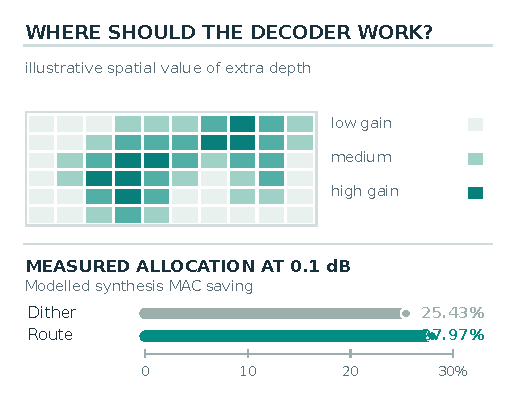
\includegraphics[width=\columnwidth]{figs/reglic_intro/reglic_intro.pdf}
\caption{\textbf{Depth is a spatial decision.} \textbf{Top:} a schematic
tile field illustrates that the value of additional synthesis can vary
within one image; colours are conceptual, not measured tile errors.
\textbf{Bottom:} at a nominal 0.1\,dB $\Delta_{444}$ target, learned
routing saves \MainRouterSaving\% of \emph{modelled synthesis MACs},
versus \MainDitherSaving\% for ordered dithering
(\MainPremium{}-point difference). These source-calibrated results are
not end-to-end latency measurements.}
\label{fig:intro}
\end{figure}

Spatial capacity selection is established in restoration: ClassSR
assigns super-resolution patches to networks of different sizes
\cite{kong2021classsr}, while APE lets patches leave a shared network
according to predicted incremental benefit~\cite{wang2022ape}.
AdaNIC brings spatially dynamic transforms to image compression
\cite{tao2023adanic}. For a codec, however, decoder depth is coupled to
the coded representation and the rate at which it was produced. A
visually complex patch need not benefit from a deeper decoder if its
bitstream carries little recoverable detail. The relevant quantity is
therefore the \emph{marginal reconstruction gain} of more synthesis,
relative to its computation and coding cost.

We study this allocation in the intra model of DCVC-UF
\cite{li2026dcvcuf}. Its twelve constant-width synthesis blocks expose
depth as a clean capacity axis without changing feature width. RegLIC
has two complementary realisations. In the
\emph{shared-exit} path, every region uses the same coded latent and
decoder prefix, then exits after a chosen block pair. In the
\emph{independent-depth} path, a selector chooses a complete 2/4/6/8/10/12-
block codec before encoding a region, allowing its analysis and entropy
models to specialise as well. The latter trades representation reuse
for specialised coding and introduces region-boundary and signalling
costs. We evaluate the shared-exit path here; the independently trained
bank is an ongoing capacity study, not a demonstrated routed system.

The evaluated design must actually \emph{skip} computation: computing
every depth and choosing an output afterwards would save no decoding
work. A full-frame stem supplies a common latent feature canvas;
conditional block pairs process a shrinking batch of active tiles.
Exit adapters align features from different depths before a shared
full-frame repair and reconstruction head. This preserves a common
output path while allowing each tile to stop at a different depth.

Separating the benefit of shallow decoding from the benefit of
\emph{placing} deeper computation is central to the evaluation.
Uniform exits and ordered dithering already reduce average depth;
the latter mixes depths without predicting which locations need them.
At a nominal 0.1\,dB YCbCr-MSE-ratio target across 53 intra frames and
five QPs, routing saves \MainRouterSaving\% of modelled synthesis MACs,
\MainPremium\ percentage points more than dithering under
per-source calibration (\cref{fig:intro}). A retrospective common
delivered-loss cap retains a margin, but when controls are fitted on
other sequences, the QP32 paired advantage is unresolved. The
arithmetic saving is consequently established more strongly than a
source-independent routing gain or complete-codec speedup.

Our contributions are a conditional DCVC-UF synthesis path with
executed tile exits; a controlled comparison that isolates spatial
placement from cheaper average depth; and a depth-bank protocol that
tests the separate question of whether independent representation
specialisation can repay its coding and boundary costs. Together they
turn synthesis depth from a fixed architectural choice into an
explicit, measurable spatial allocation problem.

\section{Related Work}
\label{sec:related}

\paragraph{Spatially adaptive reconstruction.}
ClassSR routes super-resolution patches to networks of different
capacity~\cite{kong2021classsr}; APE instead permits patches to exit a shared
network at different depths~\cite{wang2022ape}. These are direct precedents
for spatial capacity selection, so patch routing itself is not our novelty
claim. We examine the additional constraints of a coded representation:
which decision information is available at each endpoint, what must be
signalled, and how a local assignment affects final reconstruction quality.

\paragraph{Adaptive complexity in compression.}
Slimmable compressive autoencoders provide multiple model
widths~\cite{yang2021slimcae}. AdaNIC combines blockwise transform capacity
with a routing agent~\cite{tao2023adanic}, while cgSlimDecoder selects
decoder channel widths under complexity constraints~\cite{hu2023cgslim}.
These methods already establish content- or complexity-dependent computation
within learned compression. Our comparison focuses on depth allocation in
the synthesis path of a fixed coded representation and on its incremental
benefit over blind mixtures. A matched reproduction of these alternatives
remains necessary for a claim of superiority over adaptive codec designs.

\paragraph{Efficient synthesis and practical execution.}
Shallow decoders investigate how computation can be shifted toward the
encoder~\cite{yang2023shallow}. DCVC-RT distinguishes arithmetic cost from
operational overhead, including memory traffic and function
calls~\cite{jia2025dcvcrt}; DCVC-UF further develops a throughput-oriented
video codec~\cite{li2026dcvcuf}. These results motivate reporting actual
execution in addition to multiply--accumulates. Our scope is the supplied
intra model, not DCVC-UF's inter-frame or chunk-coding performance.

\paragraph{Distortion and perception.}
Generative compression explicitly studies reconstruction fidelity and
perceptual realism~\cite{mentzer2020,muckley2023illm}. A small PSNR change
therefore cannot establish perceptual equivalence. We use archived
non-DCVC experiments only to examine this limitation and the dependence on
decoder architecture; they are not evidence of a perceptual guarantee for
FLEX.

\section{Spatial Early Exit under a Quality Target}
\label{sec:method}

\subsection{Shared representation and conditional execution}
Let $\hat y$ denote the decoded latent of a fixed analysis transform and
entropy model. A full-frame upsampling stage and four shared trunk blocks
produce features with 384 channels at one eighth of the RGB resolution.
The pinned e15 configuration partitions this canvas into $32\times32$
feature tiles, corresponding to $256\times256$ RGB regions. The remaining
eight blocks are executed in pairs. Although the model exposes six nominal
exit indices, the first two lie before the split and are clamped: inference
has four distinct reachable depths, $\mathcal K=\{6,8,10,12\}$.

Each active tile traverses the next pair of blocks. Tiles assigned to that
depth pass through an exit-specific pointwise adapter and leave the active
batch; the others continue. The adapted tiles are stitched into a feature
canvas. A grid-conditioned repair and the shared output head reconstruct the
image. The halo-free tiled trunk uses replicate padding. This reduces work
only when the execution path actually removes departed tiles; evaluating all
branches and masking their outputs would have different runtime behaviour.

\subsection{Selection objective and its approximation}
For tile $t$ and exit $k$, let $M_{t,k}$ be the source MSE measured from a
candidate tiled reconstruction, and let $R$ be the source MSE of the full-depth
released-weight reference on the padded source. The search uses the table surrogate
\begin{equation}
 \widetilde\Delta(\mathbf k)=10\log_{10}
 \frac{N^{-1}\sum_{t=1}^{N} M_{t,k_t}}{R}.
 \label{eq:surrogate}
\end{equation}
The recorded cost $c_k$ is normalised to a full-frame reference decode. For
equal padded tiles, the cost model gives
\begin{equation}
 C(\mathbf k)=N^{-1}\sum_t c_{k_t},\qquad
 S(\mathbf k)=100\,[1-C(\mathbf k)].
 \label{eq:cost}
\end{equation}
Source-informed selection chooses
\begin{equation}
 k_t(\lambda)=\arg\min_k\{M_{t,k}+\lambda c_k\},
 \label{eq:search}
\end{equation}
with a per-frame search for the quality target. We call this procedure
\emph{source-informed search}, rather than a certified global optimum of the
final reconstruction problem.

The distinction is substantive. Tables are selected on the padded RGB image;
reported loss uses the final mixed reconstruction and the full-frame
\emph{fine-tuned e15} reconstruction, both cropped to the source extent.
The two anchors differ in synthesis weights as well as spatial support;
the supplement traces both evaluation paths and the checkpoint comparison.
In addition, full-frame repair and head operations couple
neighbouring tiles. Consequently, $\widetilde\Delta$ is a selection surrogate,
not an identity for delivered distortion. We report both the target and the
measured loss and count crossings of the nominal threshold explicitly.
These crossings do not isolate enforcement error under a common reference;
that requires a new evaluation against both cropped anchors.

\subsection{Router and content-blind controls}
The router projects intermediate synthesis features and latent/entropy-scale
information, pools them per tile and predicts exit scores. Given log scores
$\ell_{t,k}$, the recorded decision is
\begin{equation}
 k_t(\beta)=\arg\max_k\{\ell_{t,k}-\beta c_k\}.
 \label{eq:router}
\end{equation}
The evaluated sweep fits $\beta$ separately on each source frame's table.
This measures the attainable allocation with source calibration. Deployment
with a fixed, held-out control parameter is a separate experiment.
Increasing $\beta$ makes the selected cost non-increasing, but need not make
source distortion monotone. The supplement audits the recorded bisection
against the finite set of assignments along this control path.

Uniform depth selects one reachable exit for the whole frame. Bayer dithering
mixes two adjacent exits according to a fixed spatial ordering, with its
mixture fraction selected under the same table-based quality target. It has
no content predictor but can realise finer average costs than uniform depth.
All four methods use the same checkpoint and per-exit cost vector.

\subsection{Rate and decision information}
Keeping the coded latent fixed does not make all routing modes byte-identical.
Encoder-selected maps require a communicated decision representation. A
source-calibrated decoder router also needs its control parameter to be
communicated or otherwise reproduced. The curves in this study model decoder
MACs and do not add router cost or decision signalling to that quantity.
They therefore isolate allocation quality; a deployment comparison must
add those costs and verify actual encoded bytes separately.

\section{Results and Measurement Analysis}
\label{sec:experiments}

\subsection{Protocol}
The primary archive contains the first intra frame of 53 CTC sequences at
QP values $\{0,16,32,48,63\}$, giving 265 frame--QP pairs. We evaluate the
pinned e15 shared-latent checkpoint and one fixed router checkpoint at six
target budgets between 0.05 and 0.5\,dB. Reconstructions were produced by the
mixed tiled decoder; this revision reanalyses those outputs and does not
introduce new GPU measurements. Means compare the common cases for which
all four rules returned a plan. This leaves 204 pairs at 0.05\,dB,
263 at 0.1\,dB and 265 at each larger target. Missing plans are not silently
treated as successful full-depth fallbacks.

Paired confidence intervals resample sequences with all their available QPs
kept together, using 5,000 bootstrap draws. They describe variation over the
available content at fixed trained weights, not training-seed uncertainty.
We also repeat the budget trend on the same 204 pairs throughout to expose
the effect of changing cohort membership.

\subsection{The incremental value of content prediction}
At a 0.1\,dB target, source-informed search saves
\MainOracleSaving\% of modelled decoder MACs, the router
\MainRouterSaving\%, Bayer dithering \MainDitherSaving\%, and uniform depth
\MainUniformSaving\% (\cref{fig:budget}). The router's paired advantage over
dithering is \MainPremium\ points, with a 95\% interval of
[\MainPremiumLow, \MainPremiumHigh]. This is the incremental arithmetic value
of learned allocation under the recorded calibration procedure, not the
router's total saving against full depth.

The advantage declines as the target relaxes: it is \MediumPremium\ points
at 0.2\,dB, \LoosePremium\ at 0.3\,dB and \SaturatedPremium\ at 0.5\,dB.
The cheapest reachable exit imposes a \MacCeiling\% ceiling on this cost
model. Near that ceiling, many maps assign almost every tile to the same
exit, leaving little decision value for a content predictor. The fixed-cohort
analysis retains the declining trend, and the QP breakdown shows that its
location depends on the operating rate.

A fixed-histogram diagnostic isolates spatial placement further. For each
recorded map, we compute the exact expected table MSE after uniformly
permuting its exit assignments. This preserves the number of tiles at every
depth and hence its modelled cost. At 0.1\,dB, the router's placement improves
the table statistic by 0.0213\,dB on average (95\% interval
[0.0167, 0.0262]), while dithering gives 0.0007\,dB
([$-0.0002$, 0.0017]). These are source-table diagnostics, with the derivation
and fixed-histogram optimum in the supplement; final mixed reconstructions
would need to be decoded separately.

\begin{figure*}[t]
\centering
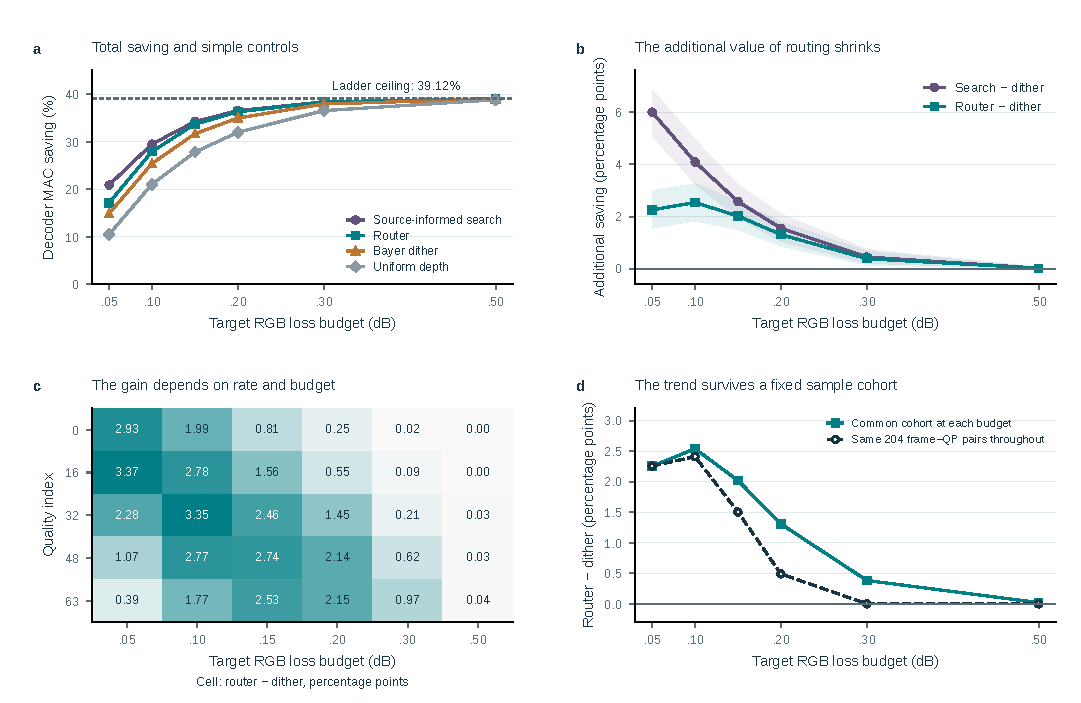
\includegraphics[width=\textwidth]{figs/refresh20260927/fig2_budget_value.pdf}
\caption{\textbf{Separate total saving from the value of routing.}
\textbf{a}, Four policies on their common cases at each target.
\textbf{b}, Paired differences with 95\% sequence-cluster bootstrap intervals.
\textbf{c}, Router--dither difference by QP and target, in percentage points.
\textbf{d}, The same comparison on a fixed cohort of 204 frame--QP pairs.
All curves use source-calibrated per-frame controls and a decoder MAC model;
they do not include router/signalling cost or constitute latency measurements.}
\label{fig:budget}
\end{figure*}

\subsection{A quality target is not a delivered guarantee}
The policies do not achieve exactly the same loss at the same nominal target
(\cref{fig:quality}a). At 0.1\,dB, the router exceeds target plus
$10^{-4}$\,dB in \MainRgbOver/\MainN\ cases in RGB and
\MainYuvOver/\MainN\ cases in YUV 6:1:1. Maximum losses are
\MainRgbMax\,dB and \MainYuvMax\,dB, respectively. These are crossings of the nominal numeric target in the exported metric,
not a clean test of a common-reference constraint: selection uses a released
anchor on padded RGB, while reporting uses the fine-tuned full-depth output
on cropped images. Metric choice and cross-tile coupling are additional
differences. The exported records cannot separate their contributions.
A framewise guarantee requires the same anchor, support and metric in
selection and final verification.

\begin{figure*}[t]
\centering
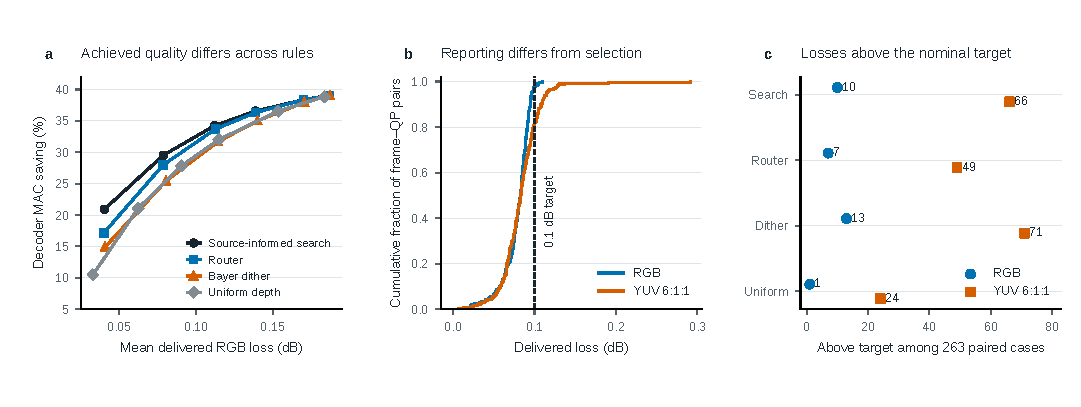
\includegraphics[width=\textwidth]{figs/refresh20260927/fig3_delivered_quality.pdf}
\caption{\textbf{Measure the reconstruction that is delivered.}
\textbf{a}, Recorded mean RGB loss against MAC saving; connected segments
guide the eye. \textbf{b}, Empirical loss distributions for the router at a
0.1\,dB target. \textbf{c}, Losses above the nominal target among 263 paired cases, measured
after cropping, with tolerance $10^{-4}$\,dB. The search used padded RGB
tables with a released-weight anchor; reporting uses the fine-tuned e15
full-depth anchor. Counts are not an isolated guarantee test. No verified
fallback was applied in this archive.}
\label{fig:quality}
\end{figure*}

\subsection{The encoder cost of knowing the source error}
The error table in \cref{eq:search} requires candidate reconstructions.
The historical QP32 benchmark recorded 1,347.65\,ms for six trial exits,
1,023.26\,ms after deduplicating the four reachable outputs, and 336.87\,ms
when a single tiled pass reused the common prefix (\cref{fig:decision}).
The last change reduces table-construction time by approximately fourfold.
These are the archived upper medians of 24 pooled trials over eight frames,
not an end-to-end encoder speedup. The raw repetition distribution and device
load history were not retained. Moreover, the archived GPU search timer can
include pending reference-decode work, so we do not use it as an isolated
search latency.

A fixed-control router can avoid the per-frame source-error table. The
source-calibrated router curves reported here cannot: they use that table to
choose $\beta$. A useful next comparison must therefore measure the complete
decision path under each information regime, including any extra stem work
at the encoder, map/control signalling and the final quality check.

\begin{figure*}[t]
\centering
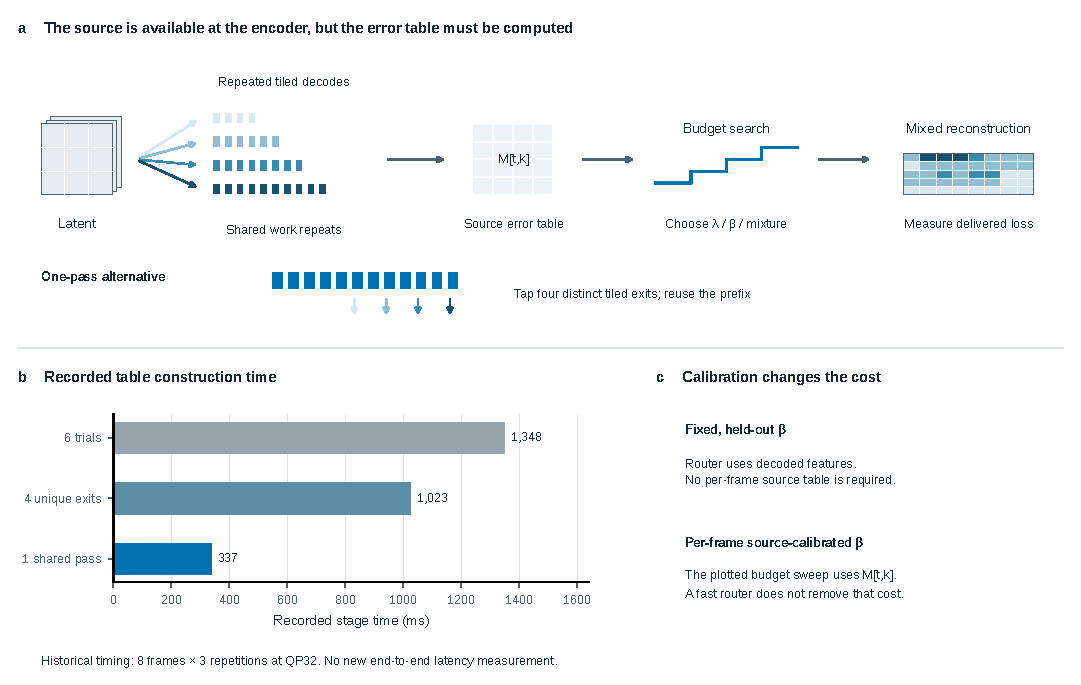
\includegraphics[width=\textwidth]{figs/refresh20260927/fig4_decision_cost.pdf}
\caption{\textbf{Obtaining the decision information has a cost.}
\textbf{a}, Candidate reconstruction, source-error tabulation, control search
and final mixed reconstruction are distinct stages. A shared pass can reuse
the trunk prefix. \textbf{b}, Archived table-construction timings; no raw
trial uncertainty is available. \textbf{c}, Fixed held-out control and
per-frame source calibration have different information requirements.
These historical stage measurements do not establish current end-to-end latency.}
\label{fig:decision}
\end{figure*}

\subsection{Spatial assignments and transfer limits}
\Cref{fig:maps} shows the recorded maps of one QP32 frame at two targets.
The example is chosen from the five archived thumbnails by proximity to the
aggregate router--dither premium at 0.1\,dB. The source thumbnail supplies
spatial context; it is not presented as a reconstruction-quality comparison.
The convergence of maps at the relaxed target illustrates the ladder's
saturation, but the aggregate claim comes from the full paired analysis.

\begin{figure*}[t]
\centering
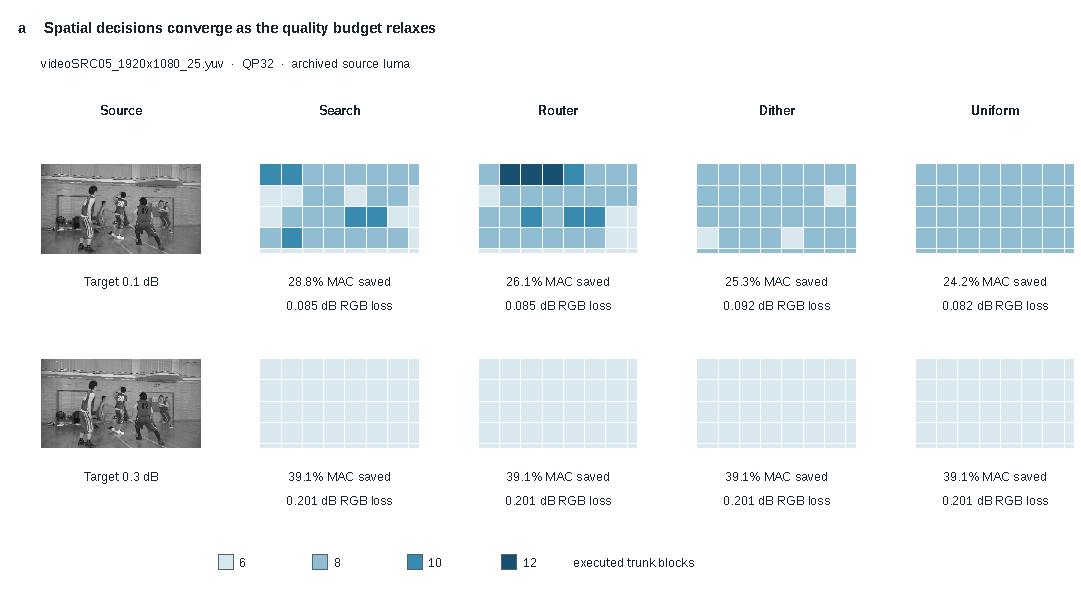
\includegraphics[width=\textwidth]{figs/refresh20260927/fig5_spatial_decisions.pdf}
\caption{\textbf{Recorded spatial decisions under two budgets.}
The left column is source luma. Other columns show actual maps, cropped to
the visible image extent, with executed depth, modelled MAC saving and
delivered RGB loss. This figure visualises allocation rather than perceptual
equivalence. The example-selection rule is stated in the text.}
\label{fig:maps}
\end{figure*}

Archived experiments on other decoders provide a useful boundary check
(\cref{fig:transfer}). Their selection criterion measures deviation from a
reference reconstruction, and their region/halo accounting models potential
compute reductions. The dense masked implementation evaluates candidates
before selection; these results therefore do not demonstrate conditional
execution speedups. The source-informed heuristic does not uniformly beat
the best blind control. Separate Kodak perceptual-budget experiments also
show that a PSNR constraint can permit appreciable LPIPS degradation.
Neither finding can be transferred into a numerical claim about DCVC-UF
without a matched experiment.

\begin{figure*}[t]
\centering
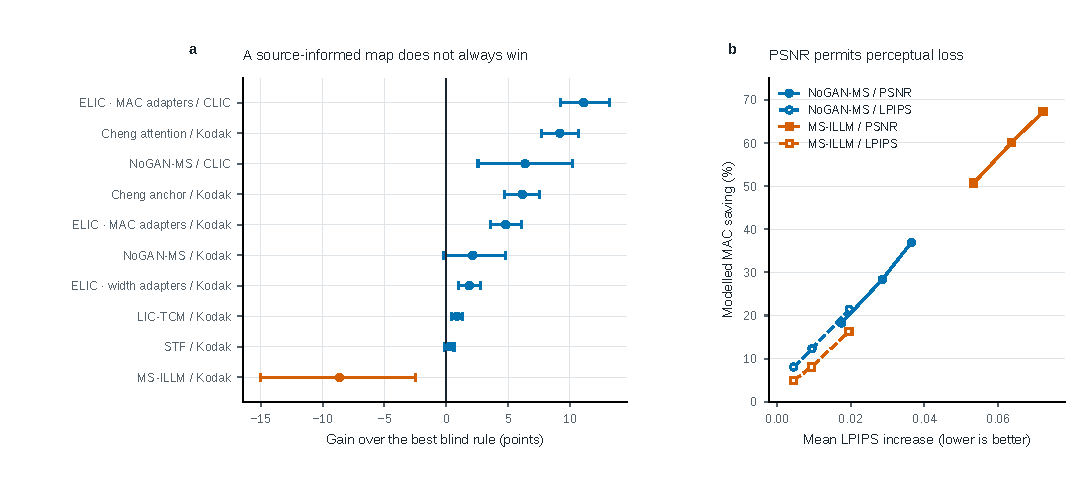
\includegraphics[width=\textwidth]{figs/refresh20260927/fig6_scope_and_perception.pdf}
\caption{\textbf{Architecture and metric limit the scope of the result.}
\textbf{a}, Source-informed selection minus the best dataset-level blind
rule at a 0.1\,dB target, with paired image-bootstrap 95\% intervals.
Adapter variants and datasets remain separate. Savings are modelled over
dense masked reconstructions. \textbf{b}, Independent Kodak-24 evaluations
under PSNR or LPIPS constraints for NoGAN-MS and MS-ILLM. The three points
per curve are recorded operating points, not interpolated observations.
These experiments use other decoders and do not validate FLEX latency or perception.}
\label{fig:transfer}
\end{figure*}

\section{From Shared Exits to Independent Depths}
\label{sec:depth}

Shared early exit commits every region to one encoded representation.
An independent codec can specialise its representation for a smaller
synthesis network, but forfeits that reuse. This motivates our complementary
2/4/6/8/10/12-block DCVC-UF bank (\cref{fig:overview}), where a later
ClassSR-inspired selector will choose a codec before encoding each region.
D2/D4/D6 are training; D8/D10 are planned and D12 is the released anchor.
No six-expert routing result is claimed.

\paragraph{A controlled capacity frontier.}
The scratch runs preserve the pinned official 105-epoch
recipe~\cite{microsoft2026training}, including all 384,795 Open Images
train\_0/1/2 images, batch size 16 and FP32. Analysis and entropy weights
learn alongside synthesis, so equal QP does not imply equal coded rate.
A frozen epoch-20 diagnostic on 100 DIV2K centre crops uses 2,000 actual
CPU bitstreams across D2/D4/D6 and released D12. At 0.2 payload bpp, D6
exceeds D2 by 0.183\,dB RGB on the 99 images with common rate support.
These interim curves establish a measurable depth frontier; final
same-recipe D12 and matched shared-exit training are still required to
attribute differences to depth or weight sharing. The supplement gives
the schedule, counts and complete curves.

\paragraph{The spatial cost of specialisation.}
Patchwise expert selection also changes geometry and entropy boundaries.
With identical D6 weights, independently coded regions lose quality at
matched rate; increasing context alone does not remove their rate cost.
In a separate fixed D2/D6 assignment, merging compatible neighbouring
regions improves matched-rate quality while retaining the same per-pixel
depth map. These controls, detailed in the supplement, make patchwise D12
and blind expert mixtures essential baselines before a selector receives
credit. The eventual comparison must match achieved rate and quality,
charge signalling and grouping, and measure the effect of expert occupancy
on latency. It will test when independent specialisation is worth more
than shared-prefix reuse.

\section{Discussion}

\paragraph{Adaptation should pay for the decisions it changes.}
FLEX-UF identifies a budget-dependent role for spatial allocation.
Under source calibration, tight quality targets leave room for useful
placement. Near the shallowest-exit ceiling, a blind mixture reaches
nearly the same arithmetic saving. This motivates a budget-conditioned choice between fixed, blind and
learned policies, with its switching rule fixed on validation data.

\paragraph{Reuse and specialisation are different commitments.}
Shared exits retain one representation and the work already performed;
independent experts can adapt their encoders and synthesis capacity more
freely. The bank adds model residency, entropy boundaries and occupancy-dependent
execution costs. Its quality must be paired with those costs, not with
shared-prefix arithmetic. Multiple exits inside each expert are outside
the present design.

\paragraph{The remaining evidence gap.}
The source-calibrated study measures available allocation value, while
the fixed-control replay leaves the routing increment unresolved.
Content-grouped calibration on untouched images is the next test of that
increment. Native bitstreams and paired wall-clock measurements must then
include entropy work, prediction, tile movement, grouping and fallback.
The current confidence intervals cover sample variation at fixed weights,
not independent training seeds. Results are confined to intra reconstruction:
YCbCr-MSE and RGB diagnostics do not establish perceptual equivalence,
temporal consistency or performance of DCVC-UF's chunk-based video path.

\section{Conclusion}
FLEX-UF makes synthesis depth a spatial decision inside DCVC-UF.
A common latent and prefix support aligned early exits, while a shrinking
tile batch turns stopping decisions into omitted block evaluations.
The measured arithmetic savings have two sources: cheaper average depth
and a smaller, budget-dependent increment from learned placement.
Blind mixtures and fixed-control replay show why these must be evaluated
separately. The independent-depth study extends the allocation question
to codec selection; matched training and complete execution measurements
will determine when specialisation justifies giving up shared computation.

\clearpage
{\small\bibliographystyle{ieeenat_fullname}\bibliography{main}}
\end{document}
